\section{TRIỂN KHAI CƠ SỞ DỮ LIỆU}
\subsection{Tổng quan về Aiven - Dịch vụ đám mây cơ sở dữ liệu}
\hspace*{1cm}
Khi triển khai một hệ thống cũng như ứng dụng, bước đầu tiên luôn là triển khai với cơ sở dữ liệu vì cơ sở dữ liệu đóng vai trò then chốt trong việc lưu trữ và quản lý thông tin. Cơ sở dữ liệu là nơi lưu trữ tất cả dữ liệu quan trọng mà ứng dụng cần để hoạt động, bao gồm thông tin người dùng, các giao dịch, và các cấu hình hệ thống. Bằng cách thiết lập cơ sở dữ liệu trước, nhà phát triển đảm bảo rằng mọi thành phần khác của ứng dụng có một nền tảng vững chắc để truy cập và xử lý dữ liệu. Điều này giúp giảm thiểu rủi ro lỗi và tăng cường hiệu suất khi tích hợp các chức năng khác của ứng dụng. Việc triển khai cơ sở dữ liệu từ sớm cũng là bước quan trọng để tất cả mọi người khi phát triển hệ thống sẽ đảm bảo được việc đồng nhất dữ liệu giữa các bên, đảm bảo tính đúng đắn của dữ liệu đối với các tác vụ đọc, thêm, sửa hoặc xóa, giúp cho quá trình phát triển hệ thống trong nhóm được hiệu quả hơn. Ngoài ra, việc triển khai cơ sở dữ liệu sớm còn cho phép kiểm thử và tối ưu hóa các truy vấn dữ liệu, đảm bảo rằng hệ thống hoạt động một cách hiệu quả và mượt mà ngay từ đầu.\\
\hspace*{1cm}
Hiện nay, có rất nhiều dịch vụ đám mây để triển khai cơ sở dữ liệu, bao gồm các dịch vụ miễn phí và có trả phí, nhưng nổi trội hơn hết vẫn là ba dịch vụ đám mây hàng đầu thế giới đó là \textit{Google Cloud}, \textit{Microsoft Azure} và \textit{Amazon Web Services}. Tuy nhiên ba dịch vụ trên đòi hỏi các bước cấu hình phức tạp khi triển khai cơ sở dữ liệu, mặc dù cả ba dịch vụ đều có hỗ trợ triển khai miễn phí tuy nhiên khả năng sử dụng lại khá hạn chế. Cho nên trong phạm vi đề tài này, sau khi đã tìm hiểu qua các dịch vụ triển khai cơ sở dữ liệu, nhóm quyết định sử dụng dịch vụ triển khai do \textit{Aiven} cung cấp. \textit{Aiven} là một nền tảng quản lý cơ sở hạ tầng dữ liệu đám mây toàn diện, cung cấp một loạt các dịch vụ cơ sở dữ liệu và dữ liệu thời gian thực như \textit{PostgreSQL}, \textit{MySQL}, \textit{Cassandra}, \textit{Redis}, \textit{Kafka}, \textit{Elasticsearch}, và nhiều dịch vụ khác. Với \textit{Aiven}, đội ngũ phát triển có thể triển khai, quản lý và mở rộng các dịch vụ dữ liệu một cách dễ dàng và hiệu quả trên các nhà cung cấp đám mây hàng đầu như \textit{AWS}, \textit{Google Cloud}, \textit{Microsoft Azure} và \textit{DigitalOcean} mà không cần lo lắng về việc quản lý cơ sở hạ tầng phức tạp. Các lợi ích chính khi triển khai cơ sở dữ liệu trên \textit{Aiven Cloud} có thể kể đến như:
\begin{itemize}
    \item \textit{Triển khai nhanh chóng:} \textit{Aiven} cho phép người dùng triển khai các dịch vụ dữ liệu chỉ trong vài phút. Điều này giúp tiết kiệm thời gian và tài nguyên, cho phép các đội ngũ phát triển tập trung vào phát triển ứng dụng thay vì phải lo lắng về việc thiết lập và cấu hình cơ sở dữ liệu.
    \item \textit{Quản lý dễ dàng:} Với giao diện người dùng thân thiện và \textit{API} mạnh mẽ, \textit{Aiven} giúp quản lý các dịch vụ dữ liệu trở nên dễ dàng hơn bao giờ hết. Các tính năng như sao lưu tự động, cập nhật phần mềm, và giám sát hiệu suất được tích hợp sẵn, giúp đảm bảo hệ thống luôn hoạt động một cách tối ưu mà không cần sự can thiệp phức tạp từ phía người dùng.
    \item \textit{Khả năng mở rộng linh hoạt:} \textit{Aiven} hỗ trợ mở rộng quy mô dịch vụ dữ liệu một cách linh hoạt. Đội ngũ phát triển có thể dễ dàng điều chỉnh tài nguyên dựa trên nhu cầu thực tế, cho phép mở rộng hoặc thu nhỏ quy mô dịch vụ mà không gây gián đoạn cho hoạt động của hệ thống.
    \item \textit{Hỗ trợ đa dịch vụ đám mây:} \textit{Aiven} cho phép triển khai các dịch vụ trên nhiều nhà cung cấp đám mây khác nhau. Điều này không chỉ tăng tính linh hoạt mà còn giúp cải thiện khả năng phục hồi của hệ thống, đảm bảo rằng dịch vụ luôn sẵn sàng ngay cả khi có sự cố xảy ra ở một nhà cung cấp đám mây nào đó.
    \item \textit{Giảm thiểu sự phức tạp}: \textit{Aiven} loại bỏ nhu cầu phải quản lý cơ sở hạ tầng phức tạp, cho phép các đội ngũ phát triển tập trung vào việc phát triển ứng dụng và dịch vụ. Điều này không chỉ giúp tiết kiệm thời gian mà còn giảm bớt gánh nặng quản lý cho các đội ngũ kỹ thuật.
    \item \textit{Hiệu suất và độ tin cậy:} Với các tính năng như sao lưu tự động, giám sát hiệu suất và cập nhật phần mềm tự động, \textit{Aiven} đảm bảo rằng các dịch vụ dữ liệu luôn hoạt động ở mức hiệu suất cao nhất. Điều này giúp cải thiện độ tin cậy và tính sẵn sàng của hệ thống, đảm bảo rằng hệ thống không bị gián đoạn trong quá trình vận hành.
    \item \textit{Bảo mật dữ liệu:} Các tính năng bảo mật mạnh mẽ của \textit{Aiven} giúp bảo vệ dữ liệu quan trọng của đội ngũ phát triển. Việc tuân thủ các tiêu chuẩn bảo mật nghiêm ngặt và hỗ trợ các công cụ xác thực hiện đại giúp ngăn chặn các cuộc tấn công và rủi ro bảo mật, đảm bảo rằng dữ liệu luôn an toàn.
    \item \textit{Lợi ích chi phí:} Bằng cách cung cấp một nền tảng quản lý dịch vụ dữ liệu toàn diện, Aiven giúp đội ngũ phát triển tối ưu hóa chi phí. Việc không cần đầu tư vào cơ sở hạ tầng phần cứng và giảm bớt yêu cầu về nhân lực kỹ thuật giúp giảm chi phí vận hành tổng thể.
\end{itemize}
\subsection{Thực hiện triển khai cơ sở dữ liệu PostgreSQL}
\hspace*{1cm}
Trong phạm vi đề tài này, nhóm sử dụng gói dùng thử \textit{Aiven Cloud} và được cung cấp số tiền là \$300.0 để sử dụng các dịch vụ. Tận dụng ưu thế này, nhóm đã sử dụng gói \textit{Startup-4} của \textit{Aiven} để triển khai cấu hình hạ tầng cho dịch vụ cơ sở dữ liệu \textit{PostgreSQL}, nhóm triển khai hạ tầng \textit{DigitalOcean} với cấu hình như sau:
\begin{itemize}
    \item \textit{CPU:} 2 \textit{CPU} cho mỗi máy ảo
    \item \textit{RAM:} 4GB \textit{RAM}
    \item \textit{Lưu trữ:} Đối với hệ quản trị cơ sở dữ liệu \textit{PostgreSQL} và \textit{MySQL}, \textit{Aiven} cung cấp dung lượng lưu trữ là 80GB.
    \item \textit{Giám sát:} Giám sát với \textit{metric} và \textit{log}
    \item \textit{Sao lưu dữ liệu:} Hỗ trợ phục hồi tại bất cứ thời điểm nào trong vòng 48 tiếng trở lại.
    \item \textit{Hạ tầng triển khai:} \textit{DigitalOcean} với rất nhiều khu vực phổ biến trên thế giới. Ở đây nhóm chọn triển khai hạ tầng ở \textit{Singapore}.
\end{itemize}
\hspace*{1cm}
Để triển khai cơ sở dữ liệu, ta cần bắt đầu với việc khởi tạo một dự án mới trong \textit{Aiven Cloud}. Mỗi dự án trong \textit{Aiven Cloud} sẽ giúp quản lý các dịch vụ được triển khai bên trong nó, thường là các dịch vụ chung cho một dự án cụ thể.
\begin{figure}[H]
    \centering
    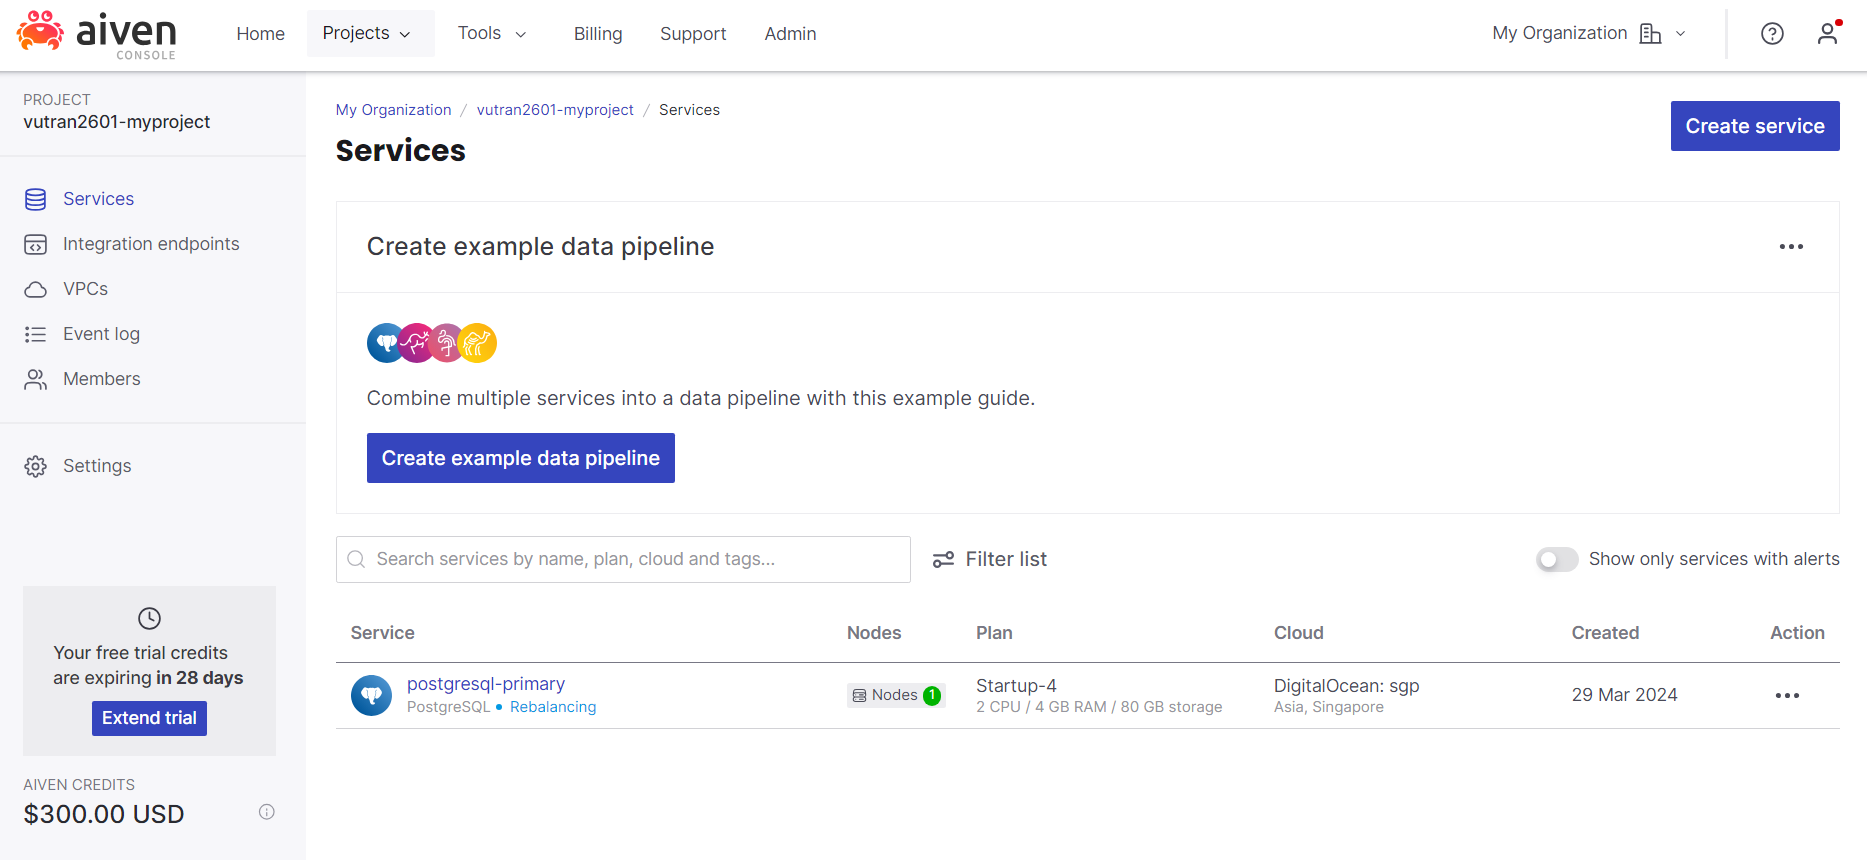
\includegraphics[width=1\textwidth]{Images/Deployment/Database/AivenProject.png}
    \caption{Khởi tạo dự án trong Aiven Cloud}
\end{figure}
\hspace*{1cm}
Bước tiếp theo sau khi khởi tạo dự án đó là cần khởi tạo dịch vụ triển khai cơ sở dữ liệu, ở đây nhóm thực hiện triển khai dịch vụ cơ sở dữ liệu \textit{PostgreSQL}. Ở trong dự án, ta cần chọn \textit{Create service} và thiết lập các cấu hình cần thiết ở các bước tiếp theo.
\begin{figure}[H]
    \centering
    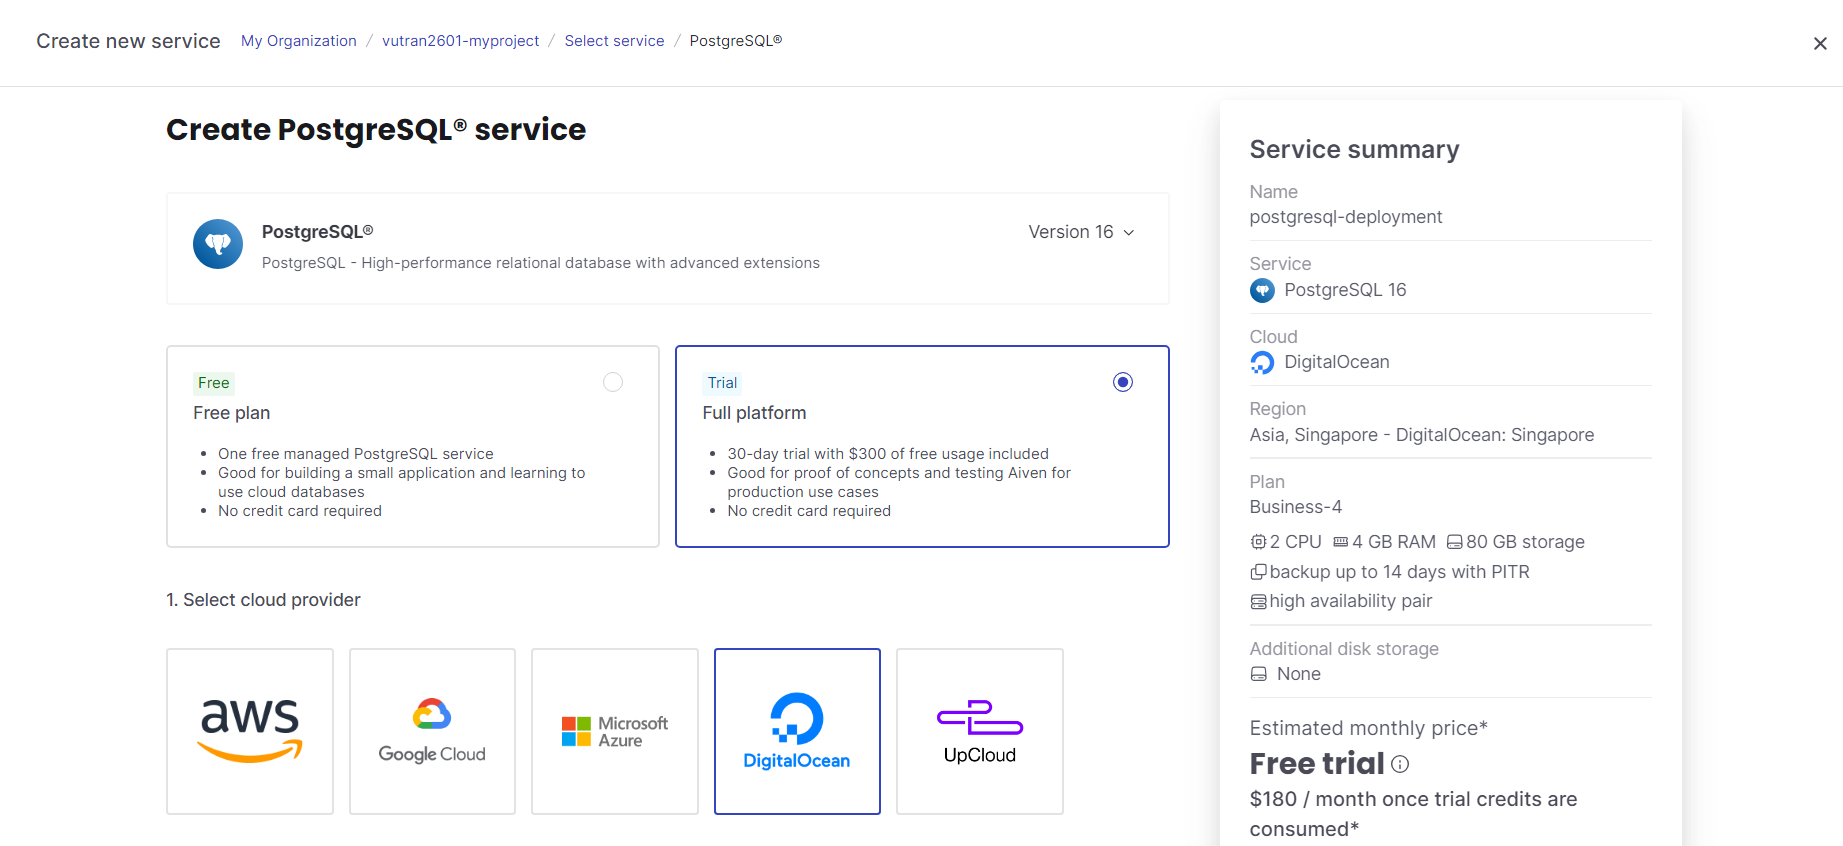
\includegraphics[width=1\textwidth]{Images/Deployment/Database/AivenConfiguration.png}
    \caption{Cấu hình khi triển khai cơ sở dữ liệu với Aiven Cloud}
\end{figure}
\hspace*{1cm}
Sau khi khởi tạo thành công dịch vụ, các bước còn lại là việc \textit{Aiven Cloud} sẽ thực hiện khởi tạo các cấu hình cho dịch vụ triển khai trên hạ tầng mà người dùng đã lựa chọn ở bước cấu hình. Ở bước này, ta cần chờ để hạ tầng thực hiện các bước cần thiết để máy chủ của dịch vụ có thể hoạt động. Sau một thời gian ngắn, dịch vụ cơ sở dữ liệu sẽ sẵn sàng để hoạt động.
\begin{figure}[H]
    \centering
    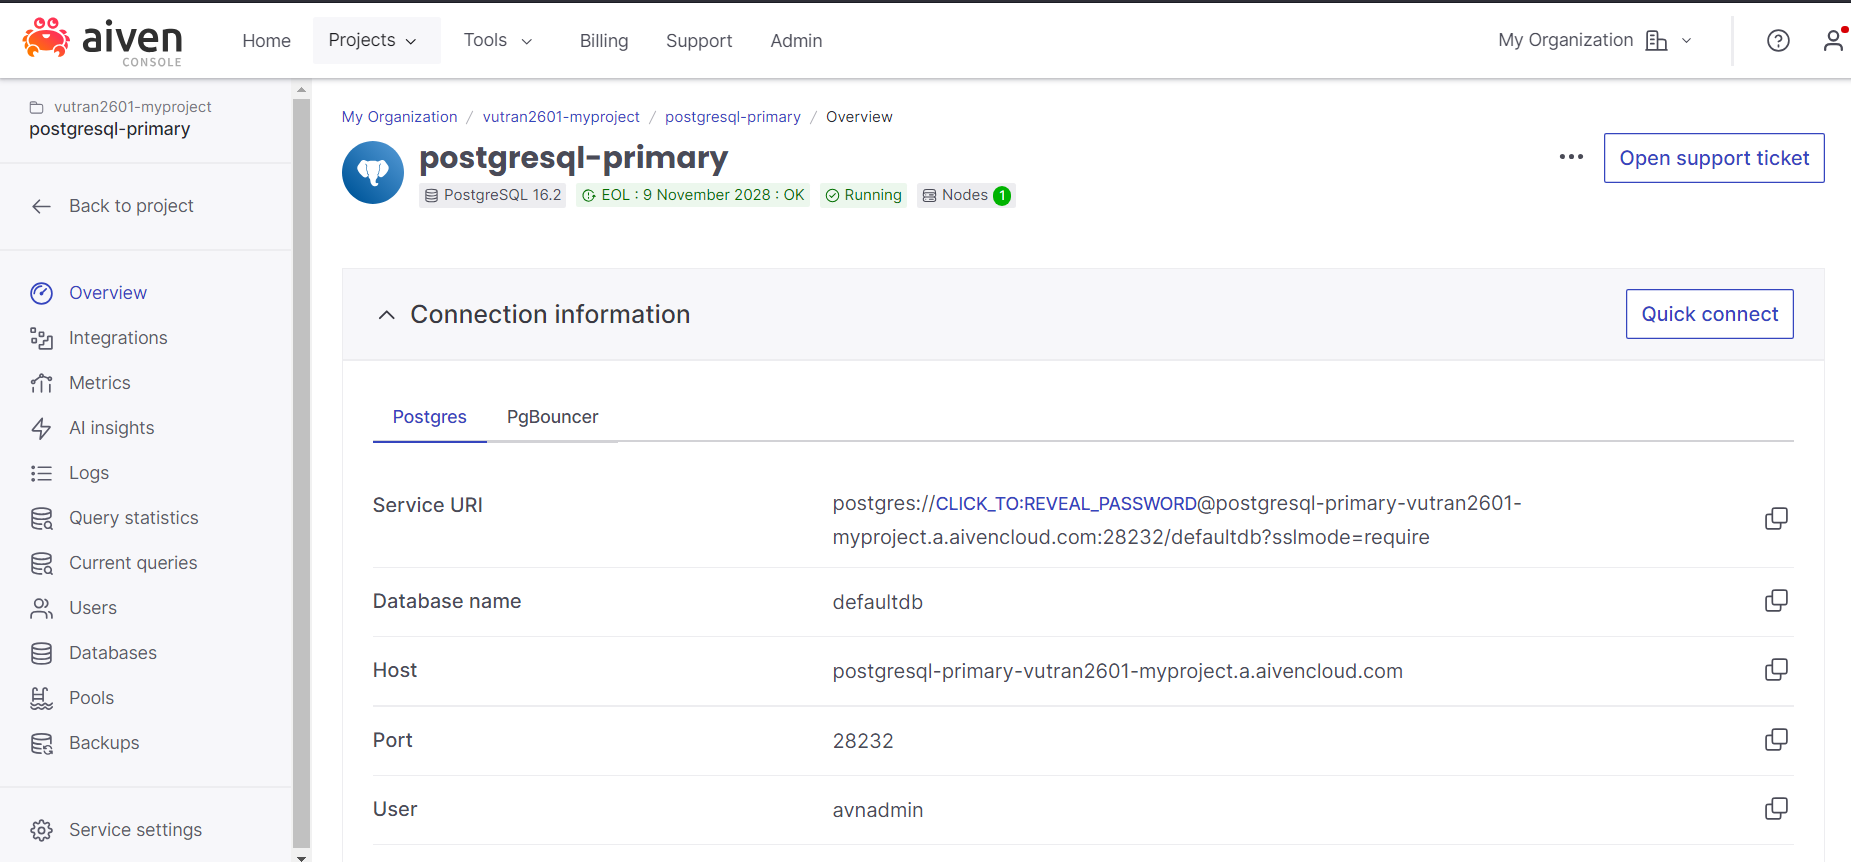
\includegraphics[width=1\textwidth]{Images/Deployment/Database/AivenRunning.png}
    \caption{Dịch vụ cơ sở dữ liệu Aiven Cloud trong trạng thái sẵn sàng kết nối}
\end{figure}
\hspace*{1cm}
Sau khi đã dịch vụ đã sẵn sàng, ta có thể kiểm tra trạng thái hoạt động của dịch vụ thông qua việc thiết lập kết nối. Ở đây ta sử dụng công cụ \textit{DataGrip}, như đã đề cập ở phía trên thì công cụ này giúp nhà phát triển có thể dễ dàng làm việc trên các cơ sở dữ liệu khác nhau. Để thiết lập kết nối với dịch vụ cơ sở dữ liệu, ở giao diện của \textit{DataGrip}, ta sẽ chọn nút dấu cộng \textit{+} ở góc bên trái phía trên và chọn \textit{Data Source}, lúc này giao diện sẽ hiển thị các loại cơ sở dữ liệu khác nhau mà \textit{DataGrip} có hỗ trợ, đến đây ta sẽ chọn \textit{PostgreSQL}. Một bảng \textit{pop-up} sẽ hiện ra và ở đây ta sẽ cần cung cấp các thông tin liên quan đến dịch vụ cơ sở dữ liệu bao gồm \textit{hostname}, \textit{port}, \textit{username}, \textit{password} và \textit{database}, sau đó ta sẽ nhấn vào \textit{Test Connection} để kiểm tra trạng thái kết nối.
\begin{figure}[H]
    \centering
    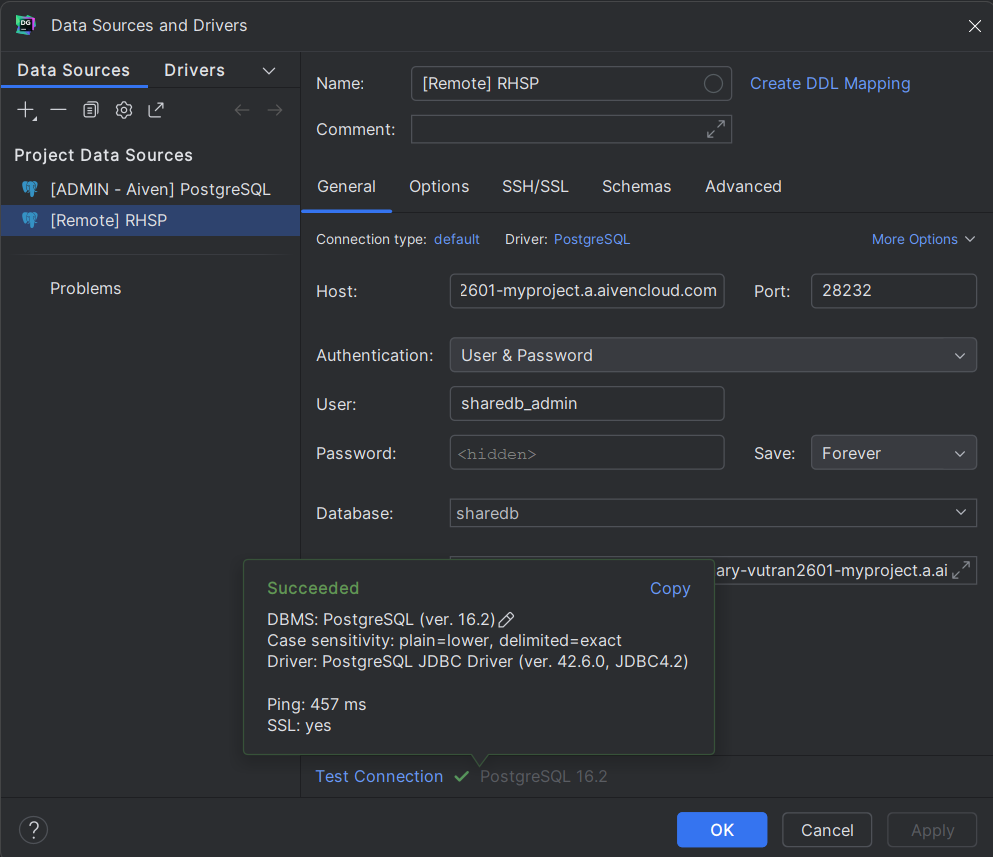
\includegraphics[width=0.8\textwidth]{Images/Deployment/Database/SuccessfulConnection.png}
    \caption{Bảng thông báo cho thấy kết nối từ DataGrip và dịch vụ Aiven Cloud đã được thiết lập thành công}
\end{figure}
